\chapter{Graph comparison \label{ch:gc}}

Graph comparison may be reduced to a problem of measuring the difference 
between two graphs. 
A primary goal of the visualization system is to allow the user to better 
verify their numerical results with visual intuition. As such, there are two 
main goals for the graph comparison output: (1) allow the user to gain some 
intuition about the qualities of the visual graph in order to better understand 
their perceptions of a ``visual trend'' in the data, and (2) provide a metric 
that quantifies the difference between the visual graph and numeric graph 
(supplied by the user). With the knowledge of both in hand, the user may 
select the numerical method which is 
``closest'' to their visual intuition and utilize the results in alternate 
applications (as in the stock selection in Chapter~\ref{ch:usage}). 
It should be noted that we operate under 
the assumption that the graphs are labeled. This avoids the sticky issue of 
isomorphism and more naturally lends itself to the visualization system's 
goals. As the VS is concerned with practical application in data 
analytics, each variable in a dataset should already correspond to some label 
(e.g. a stock).
What follows is broad overview of two graph comparison methods in 
Section~\ref{sec:gc:litreview} with more details on the graph summarization 
comparison method in Section~\ref{sec:gc:methods}. Finally, we propose a method 
to select the graph $\hat{G}^{i}, i \in \{1,...,k\}$ out of $k$ 
given graphs where $\hat{G}^{i}$ is most similar to the ``base'' 
graph $\hat{G}$ and perform a simulation study to demonstrate the method's 
viability in Section~\ref{sec:gc:simulations}. Note that we do not use the 
notation $\hat{G}^{i,\text{num}}$ for the $k$ graphs which we wish to compare 
to $\hat{G}$ because the methods discussed in this section may be 
applied to any graphs, not just numerical and visual correlation graphs.

\section{Graph summarization}
\label{sec:gc:litreview}

There are two ways of thinking about graph comparison. Let 
$\hat{G^1}=(V^1,E^1)$ and $\hat{G^2}=(V^2,E^2)$ each be some labeled graph. 

\tablespacing
\begin{enumerate}
	\item \textbf{Graph summarization:} Compute some vector 
	$v^1$ on $\hat{G^1}$ that ``summarizes'' various properties that
	it has. Similarly, compute $v^2$ on $\hat{G^2}$ to capture 
	the same properties that $v^1$ does. Finally, compute 
	$f(v^1,v^2)$ where $f$ is some distance 
	function (e.g. Euclidean distance). A high value indicates strong 
	dissimilarity while a low value indicates similarity. 
	
	\item \textbf{Graph distance:} Create a valid distance function $f$ on the 
	graphs $\hat{G^1}, \hat{G^2}$ directly rather than a vector of metrics 
	($v^1,v^2$). 
	Compute $f(\hat{G^1},\hat{G^2})$. Again, a high value indicates strong 
	dissimilarity while a low value indicates similarity. The \textit{random 
	walk kernel} is one such example of a graph distance 
	metric~\cite{vishwanathan2010}.
\end{enumerate}
\bodyspacing

We specifically focus on the graph summarization comparison because it 
fulfills both desired criteria for the visualization system; an understanding 
of each summarization method allows the user to gain intuition on the qualities 
of the graph, and the difference between two graph summarization methods can be 
quantified easily. To be more specific, we seek to better understand the 
qualities of existing graph summarization methods and their associated 
advantages and disadvantages. 
Understanding these metrics is important due to the complex nature of graphs.
It is natural to ask why we cannot just plot the graphs instead (which are 
typically in the form of either an adjacency matrix of list of edges) and 
examine the result for visual patterns in order to understand the qualities 
of the graph. This is unfeasible for several reasons (see 
Figure~\ref{fig:gc:arr_density}). 

\tablespacing
\begin{itemize}
	\item \textbf{Arrangement:} Different arrangements of nodes on the visual 
	plane may have a profound effect on the interpretability of the graph; from 
	the start, it is unclear what the best arrangement might be, and it is 
	unfeasible for an analyst to try all possible arrangements 
	especially as the number of variables increase.
	
	\item \textbf{Density:} The more nodes there are, the more edges there may 
	be, and the more dense a graph may become, making it incredibly difficult 
	to interpret. Furthermore, it makes it more difficult to find anomalies 
	among the variable's relationships (represented by edges). A non-existent 
	edge in a dense graph is just as important as an existent edge in a sparse 
	graph because each indicates a relationship which isn't quite like all the 
	others.
\end{itemize}
\bodyspacing

\begin{figure}[htb]
	\begin{center}
		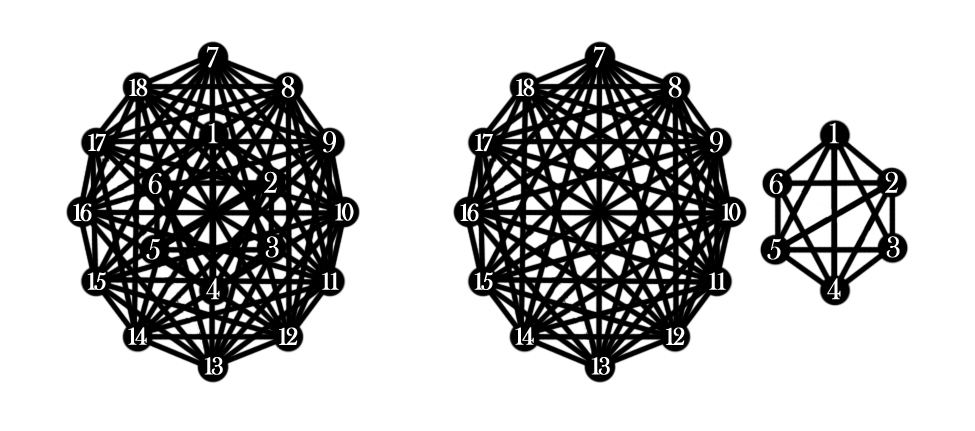
\includegraphics[width=1\linewidth]{ch-gc/figures/arr_density}
		\caption[Difficulties with graph visualization.]{
		Suppose we have a graph $G=(V,E)$ with clusters $C^1,C^2$ and $|V|=18$. 
		Let $C^1$ be composed of nodes $(V_1,...,V_6)$, and $C^2$ be composed 
		of nodes $(V_7,...,V_{18})$. 
		\textit{Left:} $C^1$, the smaller cluster, has been placed inside 
		$C^2$, the larger cluster. It is difficult to discern any meaningful 
		patterns; each node appears to be connected to every other node as the 
		density of the cluster $C^2$ makes it almost impossible to see that of 
		$C^1$.
		\textit{Right:} The nodes have been rearranged in a manner that clearly 
		distinguishes between $C^1$ and $C^2$. At a glance, it is evident that 
		$C^1$ is missing $E_{3,6}$. It is difficult to tell, however, that 
		$C^2$ is even missing an edge $(E_{13,17})$ in the first place!
		$C^1$ is more sparse, which makes it easier to visually perceive 
		anomalies in the graph.}
		\label{fig:gc:arr_density}
	\end{center}
\end{figure}

Graph summarization acts as a proxy for visually exploring the graph 
itself. Each metric, which is associated with a different characteristic of the 
graph, can be parsed and later combined to 
``reconstruct'' or better understand the qualities of each graph, subsequently 
allowing the user to better understand \textit{exactly where} the visual and 
numeric graphs differ (should the final graph comparison metric suggest that 
the two graphs are highly different). Graph distance functions skip that 
critical step by going through 
the graphs directly.

To put it in another way, graph summarization has the \textit{exact opposite 
problem} that is present in data analytics as it is practiced today (discussed 
in Chapter~\ref{ch:intro}, this is the motivation behind the VS and this 
thesis). 
The visualization system allows the user to use the visual qualities of pairwise
scatter plots to better understand numerical qualities of the data, but graph 
summarization allows the user to use numerical qualities to better understand 
the visual qualities of a graph. 

With an understanding of the properties of various graph summarization methods, 
the graph summarization difference metric may be more informative. In the VS, 
the graph summarization difference computes a list of graph summarization 
metrics $(m^\text{num},m^\text{vis})$ for each graph in order to provide a 
single vector $d$ that quantifies the difference between them with 
some difference function (e.g. Euclidean distance, L2, etc.). 
As such, a natural byproduct of the computation is 
$(m^\text{num},m^\text{vis})$, which (armed 
with an understanding of the values) provides insight on the qualities of the 
visual graph and numerical graph \textit{on an individual level} and where 
exactly their differences and similarities lie.
\section{Overview of graph summarization methods}
\label{sec:gc:methods}

\subsection{Centrality}

\subsection{Community}

\subsection{Distance matrix}

\subsection{Assortativity}

\subsection{Edge density}

\subsection{Edge connectivity}
\section{Similarity selection}
\label{sec:gc:simulations}

Given a set of $k$ graphs $\hat{G^i}$ for $i \in \{1,...,k\}$, we would like to 
select the graph $\hat{G^*}$ which is most similar to the ``base'' graph 
$\hat{G}$. Each of the $k$ given graphs are associated with a vector 
$d^{i}$ of their difference to $\hat{G}$. Each element $d^{i}_m$ for $m \in 
\{1,...,10\}$ corresponds to one of the ten summarization methods listed 
earlier in Section~\ref{sec:gc:methods} (different flavors of 
centrality and community are included). 
We propose the following methodology to select the most similar graph pair:

\tablespacing
\begin{enumerate}
	\item Compare each difference metric $d^{i}_m$ against 
	$d^{i'}_m$ for all $m \in \{1,...,6\}$ and $i,i' \in 
	\{1,...,k\}$ where $i \neq i'$. 
	\item Select the index $i$ which has the most number of smallest 
	differences. In other words, find
	$$\max\limits_{i \in \{1,...,k\}} 
	\sum\limits^{10}_{m=1} \textbf{1}_{d^{i}_m > d^{i'}_m} \ \text{where} \ i 
	\neq i' \in \{1,...,k\}$$
\end{enumerate}
\bodyspacing

Aside from returning the most similar graph pair, the proposed similarity 
selection method further eliminates the need to normalize the resulting 
difference metrics (which will not be on the same scale within the vector
$d^i$), as it compares each metric to its own metric rather 
than using $d^i$ to compute a scalar ``difference'' between graphs 
$\hat{G}^i$ and $\hat{G}$. In the next section, we demonstrate the viability of 
this strategy with a simulation study. This method is later applied in 
Chapter~\ref{ch:usage} to compare the visual correlation graph (formed from the 
VS) with the various numerical correlation graphs (formed from the correlation 
coefficients described in Section~\ref{sec:intro:correlation}).
The similarity selection method is coded in 
Appendix~\ref{sec:appendicies:gc:similarity}.

\subsection{Simulation study}
\label{sec:gc:simulations:algorithm}

We now perform a simulation study to demonstrate the viability of the proposed 
selection strategy. Let $G=(V,E)$ be a base graph with $|V|=20$ nodes and 
$|E|=50$ edges. The idea is to generate two random graphs $G^1, G^2$ from $G$ 
such that $\text{diff}(G,G^1) << \text{diff}(G,G^2)$ or vice versa. 
In other words, one graph should clearly be similar to $G$ while the other is 
very dissimilar to $G$. This is achieved by randomly swapping $\frac{|E|}{5} = 
10$ and $|E| = 50$ edges from $G$ to build $G^1$ and $G^2$, respectively. 
The random swapping algorithm is as follows:

\tablespacing
\begin{algorithm}[H]
	\caption{Random edge swapping}\label{alg:gc:simulations:swapping}
	\begin{algorithmic}[1]
		\Procedure{}{$G=(V,E)$ is the ``base'' graph. Generate a 
		random graph $G^i=(V,E^i)$ by randomly swapping $e$ edges of $G$.
		Let $p_k$ be the probability of randomly selecting node $V_k$. }
		\State $G^i \gets G$
		\State \textbf{loop from} $f=1$ \textbf{to} $e$:
		\State \indent Select an edge uniformly at random and delete from $G^i$
		\State \indent Select $V_i$ uniformly at random
		\State \indent Select $V_j$ at random where 
		$p_k = \frac{\text{deg}(V_k)}{\sum\limits_{x=1}^{|V|} \text{deg}(V_x)} 
		\ \forall \
		k \in \{1,...,|V|\}$
		\State \indent \textbf{while} ($V_i == V_j$ \textbf{or} edge 
		$(V_i,V_j)$ exists):
		\State \indent \indent Reselect $V_j$ at random with the PDF given 
		earlier*
		\State \indent Add edge $(V_i,V_j)$ to $G^i$
		\State \textbf{return} where($p==\min{(p)}$)
		\EndProcedure
	\end{algorithmic}
	*Selecting the second node in this manner ensures that the assortativity 
	coefficient continues to evolve as the swapping proceeds. 
\end{algorithm}
\bodyspacing

\noindent Naturally, $G^1$ is more similar to $G$ since less 
edges are being swapped than in $G^2$. The differences between the pair 
$(G,G^i)$ for $i \in \{1,2\}$ are computed with the summarization 
methods discussed in Section~\ref{sec:gc:methods}, and the most similar 
graph is selected with the similarity selection method described in 
Section~\ref{sec:gc:simulations}. 
The results are recorded for 1000 trials, and an average is computed. 
The code for the simulation study may be found in 
Appendix~\ref{sec:appendicies:gc:simulations}. 

\subsection{Results}
\label{sec:gc:simulations:results}

The results are summarized in Table~\ref{tab:gc:simulations}.

\tablespacing
\begin{longtable}{p{0.15\linewidth} p{0.25\linewidth} 
p{0.15\linewidth} p{0.15\linewidth}}
	
	% First page heading
	\caption[Summary of similarity selection simulation results.]{A summary of 
	the  similarity selection simulation results as described in 
	Section~\ref{sec:gc:simulations:algorithm}. The table summarizes the 
	probability of selecting graphs $G^1$ and $G^2$ with the given number of 
	swaps. (C) is an abbreviation for (CONTROL)} 
	\label{tab:gc:simulations}\\
	\toprule
	\textbf{Distance} & \textbf{Number of swaps} & 
	\textbf{Prob}($G^1$) & \textbf{Prob}($G^2$) \\
	\midrule
	\endfirsthead
	
	% Future page heading
	\caption[]{(continued)}\\
	\toprule
	\textbf{Distance function} & \textbf{Number of swaps} & 
	\textbf{Prob}($G^1$) & \textbf{Prob}($G^2$) \\
	\midrule
	\endhead
	
	% Page footer
	\midrule
	\multicolumn{4}{r}{(Continued on next page)}\\
	\endfoot
	
	% Last page footer
	\bottomrule
	\endlastfoot
	
	Euclidean & $G^1: 10, G^2: 10$ (C) & 
	0.54 & 0.46 \\
	
	& $G^1:10, G^2: 50$ & 0.885 & 0.115 \\
	
	\cmidrule[0.1pt](l{0.5em}r{0.5em}){1-4}	
	
	L1 & $G^1: 10, G^2: 10$ (C) & 
	0.532 & 0.468 \\
	
	& $G^1:10, G^2: 50$ & 0.886 & 0.114 \\
	
	\cmidrule[0.1pt](l{0.5em}r{0.5em}){1-4}	

	L2 & $G^1: 10, G^2: 10$ (C) & 
	0.541 & 0.459 \\
	
	& $G^1:10, G^2: 50$ & 0.885 & 0.115 \\
		
\end{longtable}
\bodyspacing

\noindent Though the control is slightly skewed towards $G^1$, it is still 
clear that, on average, the proposed similarity selection method is more likely 
to properly select $G^1$, the actual ``most similar graph''. To visualize 
the differences between 10 vs 10 and 10 vs 50 swaps, please review 
Figures~\ref{fig:gc:sim10vs10} and~\ref{fig:gc:sim10vs50}, which plot $G, G^1,$ 
and $G^2$ from the final simulation trial. Because the control and the regular
simulations were run separately and because each trial is seeded with 
its trial number, $G$ and $G^1$ (which has 10 swaps in each 
simulation) are the same in Figures~\ref{fig:gc:sim10vs10} 
and~\ref{fig:gc:sim10vs50}; only $G^2$ differs.

\begin{figure}[htb]
	\begin{center}
		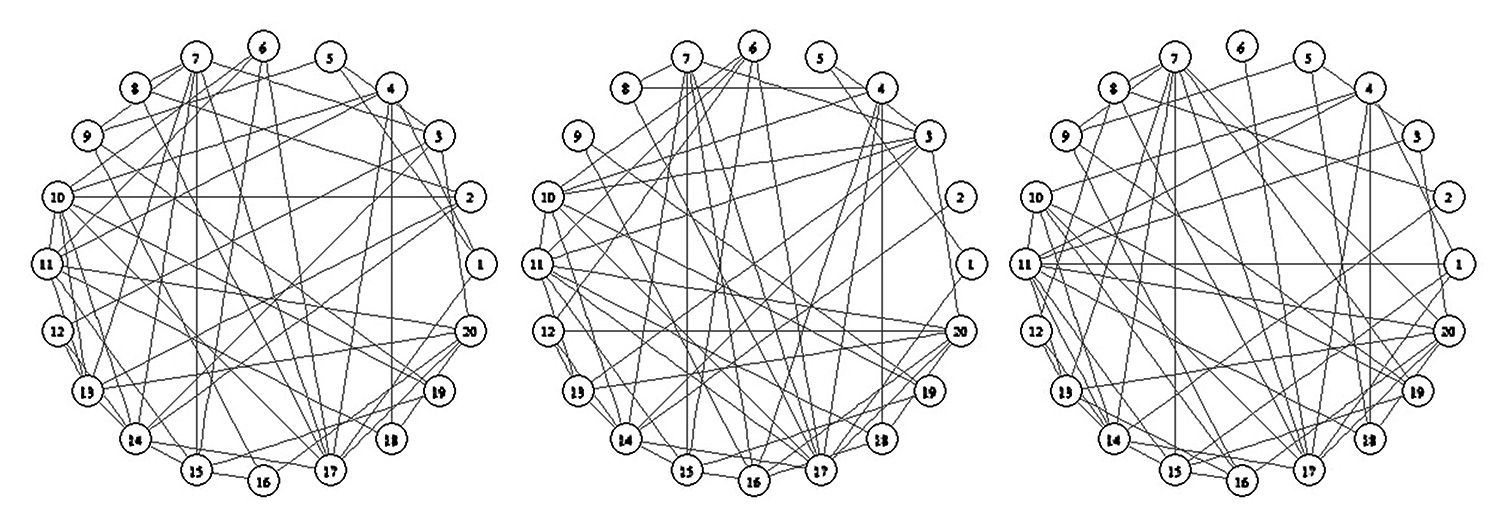
\includegraphics[width=1\linewidth]{ch-gc/figures/sim_10vs10}
		\caption[Random graphs with 20 nodes and 50 edges. Edges have been 
		swapped 10 times each.]{\textit{Left:} Base graph $G=(V,E)$ with 
		$|V|=20$ nodes and $|E|=50$ edges. 
		\textit{Middle:} Random graph $G^1$ built from $G$ by swapping 
		10 edges. \textit{Right:} Random graph $G^2$ built from $G$ by 
		swapping 10 edges. Distance: L2. Seed: 1000}
		\label{fig:gc:sim10vs10}
	\end{center}
\end{figure}

\begin{figure}[htb]
	\begin{center}
		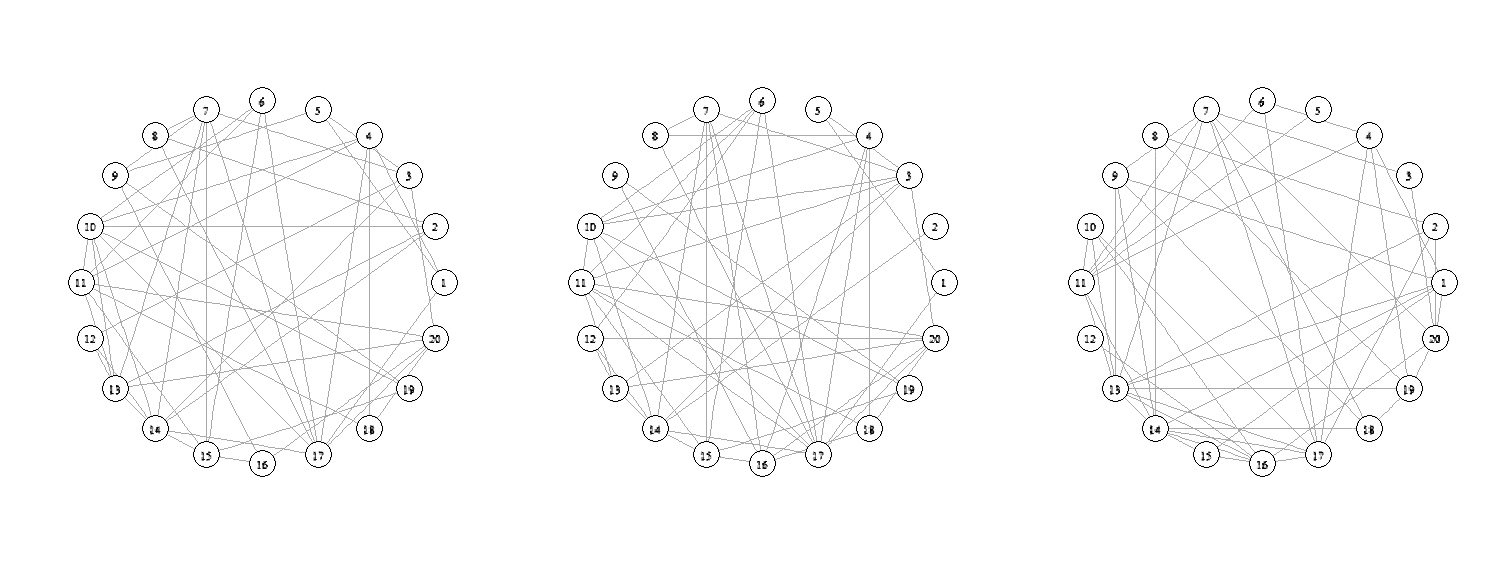
\includegraphics[width=1\linewidth]{ch-gc/figures/sim_10vs50}
		\caption[Random graphs with 20 nodes and 50 edges. Edges have been 
		swapped 10 and 50 times, respectively.]{\textit{Left:} Base graph 
		$G=(V,E)$ with $|V|=20$ nodes and $|E|=50$ edges.\textit{Middle:} 
		Random graph $G^1$ built from $G$ by swapping 10 edges. 
		\textit{Right:} Random graph $G^2$ built from $G$ by swapping 
		50 edges. Distance: L2. Seed: 1000}
		\label{fig:gc:sim10vs50}
	\end{center}
\end{figure}

\subsubsection{Extensions}

Although the normalization methods proposed in Section~\ref{sec:gc:methods} 
have bounded the individual graph summarization metrics between 0 and 1, these 
metrics are not necessarily uniformly distributed between 0 and 1. An 
alternative method of normalization utilizes the Erdos-Renyi model (which 
generates a random graph by creating every edge with the same probability) to 
normalize the \textit{overall difference metric} between 
two existing graphs $G^1=(V,E^1)$ and $G^2=(V,E^2)$. While this does not 
actually yield a scalar difference metric, the result provides insight on 
the significance of the resulting difference metric.
Let $d = \text{diff}(G^1,G^2)$. Then the procedure is as follows:

\tablespacing
\begin{algorithm}[H]
	\caption{Alternative graph difference 
	normalization procedure}\label{alg:gc:simulations:extension}
	\begin{algorithmic}[1]
		\Procedure{}{$G^1=(V,E^1)$ and $G^2=(V,E^2)$. Let $d = 
		\text{diff}(G^1,G^2)$. $n$ is the desired number 
		of trials e.g. $n = 1000$. }
		\State \textbf{loop from} $i=1$ \textbf{to} $n$:
		\State \indent Generate an Erdos-Renyi graph $\hat{G^1}$ with 
		$|V|$ nodes and $|E^1|$ edges.
		\State \indent Generate an Erdos-Renyi graph $\hat{G^2}$ with 
		$|V|$ nodes and $|E^2|$ edges.
		\State \indent $t_i \gets \text{dist}(\hat{G^1},\hat{G^2})$
		\State Compare $d$ to the empirical distribution $\{t_1,...,t_n\}$*
		\EndProcedure
	\end{algorithmic}
\end{algorithm}
\bodyspacing
 
\noindent *Compare $d$ to the empirical distribution $\{t_1,...,t_n\}$ by 
computing a $p$-value
$$\frac{\#\{t_i : t_i\geq d \}}{n}$$

\noindent for an upper tail distribution and a $p$-value
$$\frac{\#\{t_i : t_i \leq d \}}{n}$$

\noindent for a lower tail distribution. The $p$-values may be computed using 
the similarity selection methodology 
presented in Section~\ref{sec:gc:simulations}. A lower $p$-value 
suggests that $d$ is more significant (i.e. the computed difference metric is 
reliable) because it indicates that $d$ has a low probability of being an 
``extreme'' event.